% ==================== Header ====================
\documentclass[12pt]{article} %montserrat fonts exists only in 10pt-12pt
\usepackage[a4paper, top=10mm, bottom=10mm, left=12mm, right=12mm]{geometry}
\usepackage[most]{tcolorbox}
\usepackage[hidelinks]{hyperref}
\usepackage[defaultfam,tabular,lining]{montserrat}
\usepackage{enumitem}
\usepackage{dirtytalk}
\usepackage{fontawesome5}
\usepackage{numprint}
\usepackage{setspace}

% ==================== Global settings ====================
\npdecimalsign{,} % Comma for decimals (European style)
\npthousandsep{.} % Dot for thousands (European style)
\setlength{\parindent}{0mm} % No paragraph indent
\pagenumbering{gobble} % No page numbering
\hyphenpenalty=100000 % No implicit hyphens
\exhyphenpenalty=100000 % No explicit hyphens
\tolerance=5000 % Avoid bad spacing
\emergencystretch=1em % Allow minor overshoots (trust me, looks better)

% ==================== Custom commands ====================
\definecolor{custom_blue}{RGB}{2,132,199}

\definecolor{linkedin_blue}{RGB}{10,102,194}

\newcommand{\NameText}[1] {{\Large\textbf{#1}}}

\newcommand{\HighlightedText}[1] {{\textbf{#1}}}

\newcommand{\PlaceAndTime}[2] {\HighlightedText{#1} \hfill \HighlightedText{#2}}

\newcommand{\SymbolAndLink}[3] {#1 \hspace{0mm} \href{#3} {\underline{#2}}}

\newcommand{\SymbolAndText}[2] {#1 \hspace{0mm} #2}

\newenvironment{ItemizeSection}[1]{
    \vspace{1mm}
    \HighlightedText{#1}
    \vspace{0.5mm}
    {\color{custom_blue} \hrule}
    \begin{itemize}[left=0.5em, topsep=0pt, itemsep=0pt, label={$\bullet$}]
}{
    \end{itemize}
}

\newenvironment{TextSection}[1]{
    \vspace{1mm}
    \HighlightedText{#1}
    \vspace{0.5mm}
    {\color{custom_blue} \hrule}
    \begin{itemize}[left=0.5em, topsep=0pt, itemsep=0pt, label={}]
}{
    \end{itemize}
}

\newenvironment{ItemizeSubsection}{
    \begin{itemize}[left=0.5em, topsep=-999pt, itemsep=0pt, label={$\circ$}]
}{
    \end{itemize}
}

% ==================== Name and Contact ====================

\begin{document}
\setstretch{1.5} % Spacing for the header
\begin{tcolorbox}[sharp corners=all, colback=custom_blue, coltext=white, frame empty, left=2mm, right=2mm, top=1mm, bottom=1mm]

    \noindent \begin{minipage}{0.6\textwidth}
        \NameText{Kyrylo Sovailo}

        \begin{tabular}{@{}ll@{}}
            \SymbolAndLink{\faAt}{k.sovailo@gmail.com}{mailto:k.sovailo@gmail.com} &
            \SymbolAndLink{\faPhone*}{01763 5479038}{tel:+4917635479038} \\
            \SymbolAndLink{\faGithub}{github.com}{https://github.com/kyrylo-sovailo} &
            \SymbolAndLink{\faLinkedin}{linkedin.com}{https://linkedin.com/in/kyrylo-sovailo-19b4541b9} \\
            \multicolumn{2}{@{}l@{}}{\SymbolAndText{\faEnvelope}{Pallaswiesenstr. 39, 64293 Darmstadt}} \\
            %\multicolumn{2}{@{}l@{}}{\SymbolAndText{\faAddressCard}{Staatsangehörigkeit: Ukraine}} \\
            %\multicolumn{2}{@{}l@{}}{\SymbolAndText{\faBabyCarriage}{Geboren am 08.10.2000 in Kiew, Ukraine}}
            \multicolumn{2}{@{}l@{}}{\SymbolAndText{\faBabyCarriage}{Geboren am 08.10.2000}}
        \end{tabular}

    \end{minipage}
    \begin{minipage}{0.39\textwidth}
        \raggedleft
        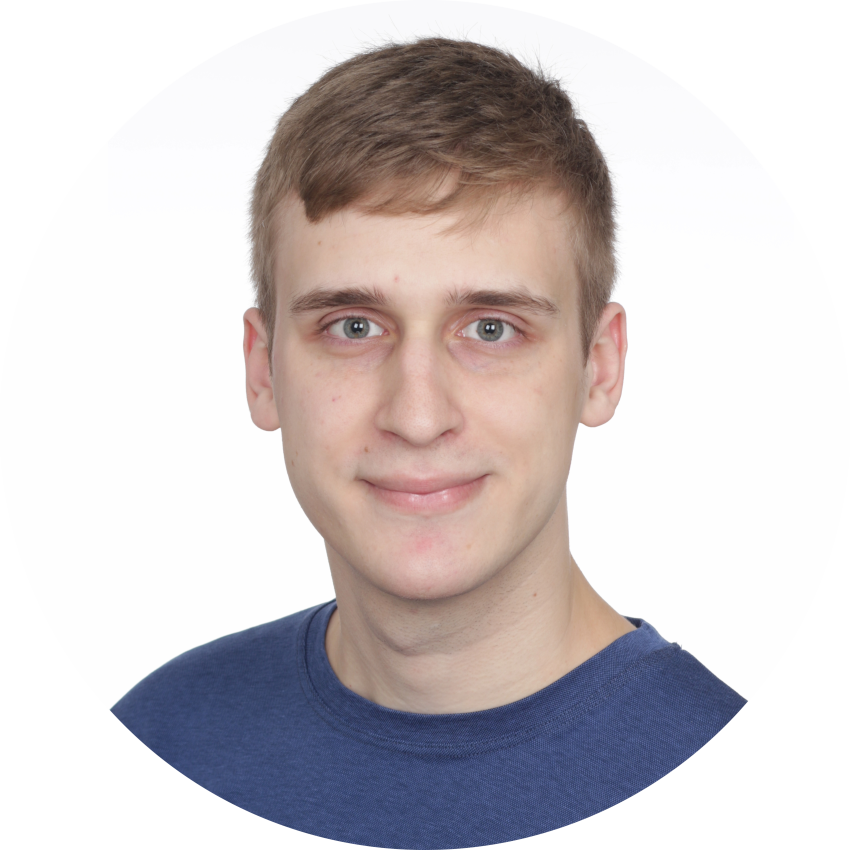
\includegraphics[width=50mm]{../images/Photo_compressed_round.png}
    \end{minipage}
\end{tcolorbox}
\setstretch{1.1} % Spacing for the rest of the document

% ==================== Education ====================
\vspace{-2.5mm}
\begin{ItemizeSection}{Ausbildung}
    \item \PlaceAndTime{Computational Engineering (CE) M.Sc.}{04.2023 -- 12.2025} \\
    \textbf{(Vertiefung Computational Robotics)} \\
    TU Darmstadt (Abschlussnote \numprint{2.1}) \\
    Abschlussarbeit (Note \numprint{1.7}):
    \begin{ItemizeSubsection}
        \item Thema: Integration von räumlicher Wahrnehmung in embeddings-basierte Anomalieerkennungsmethoden für die automatisierte industrielle Inspektion
        %\item Institut: Simulation, Systemoptimierung und Robotik (SIM)
        \item Ergebnis: Anomalieerkennungsmethode mit einer Genauigkeit von 95\% durch Kombination klassischer Algorithmen mit Foundation Models entwickelt (Python, PyTorch, Transformers)
    \end{ItemizeSubsection}

    \item \PlaceAndTime{Computational Engineering Science (CES) B.Sc.}{10.2018 -- 04.2023} \\
    RWTH Aachen University (Abschlussnote \numprint{2.4}) \\
    Abschlussarbeit (Note \numprint{1.7}):
    \begin{ItemizeSubsection}
        \item Thema: Balancierung eines 2D inversen Pendels mit Franka Panda Roboterarm
        %\item Institut: Institut für Data Science im Maschinenbau (DSME)
        \item Ergebnis: Steuerungsalgorithmen mit inverser Kinematik und Dynamik entwickelt, die dem Roboter ermöglichten, ein inverses Pendel mit zwei Freiheitsgraden zu balancieren (ROS, C++, Python)
    \end{ItemizeSubsection}

    \item \PlaceAndTime{Abitur}{09.2017 -- 09.2018} \\
     Studienkolleg an Freier Universität Berlin, technischer Kurs

    %\item \PlaceAndTime{Abitur}{09.2010 -- 05.2017} \\
    %Technisches Lyzeum der Nationalen Technischen Universität der Ukraine \say{Kiew Polytechnisches Institut}
\end{ItemizeSection}

% ==================== Professional background ====================
\begin{ItemizeSection}{Berufspraktische Erfahrungen}
    \item \PlaceAndTime{Studentische Hilfskraft an der Goethe Universität Frankfurt}{06.2023 -- 07.2024} \\
    Buchmann Institute for Molecular Life Sciences (BMLS)
    \begin{ItemizeSubsection}
        \item Grafische Slicing-Software entwickelt und die für einen Bio-3D-Drucker spezifischen Funktionen implementiert (C\#, C++, Slic3r)
        \item Software für die Druckersteuerung auf die neue Hardware portiert (C++, Arduino)
    \end{ItemizeSubsection}

    \item \PlaceAndTime{Praktikum bei Continental AG}{03.2022 -- 05.2022}
    \begin{ItemizeSubsection}
        \item Tool zur Generierung von C-Quellcode aus der CAN-Datenbank entwickelt (Python, C, CAPL)
        \item Build-Prozess der Software für einen V850-Mikrocontroller automatisiert (CMake, Python)
    \end{ItemizeSubsection}

    \item \PlaceAndTime{Studentische Hilfskraft an der RWTH Aachen University}{04.2021 -- 12.2021} \\
    Institut für Data Science im Machinenbau (DSME)
    \begin{ItemizeSubsection}
        \item High-Level-APIs für einen Franka-Panda-Roboterarm implementiert und Steuerungsalgorithmen entwickelt (Echtzeit-Linux, C++, Python)
        \item Eigenständige (ROS-unabhängige) Simulationssoftware für den Arm entwickelt (C++, Gazebo)
    \end{ItemizeSubsection}
\end{ItemizeSection}

\newpage
% ==================== Skills ====================
\begin{ItemizeSection}{IT-Kenntnisse}
\item Programmiersprachen:
    \begin{ItemizeSubsection}
        \item C, C++
        \item C\#
        \item Python
    \end{ItemizeSubsection}
    \item Entwicklungstools:
    \begin{ItemizeSubsection}
        \item CMake
        \item Git
        \item Docker
        \item Visual Studio, Visual Studio Code
        \item MATLAB/Simulink
    \end{ItemizeSubsection}
    \item Embedded-Plattformen:
    \begin{ItemizeSubsection}
        \item Atmel AVR
        \item Renesas V850
        \item STM32
        \item Teensy
        \item Raspberry Pi (Linux)
        \item NVIDIA Jetson (Linux)
        \item x86\_64 (Echtzeit-Linux)
    \end{ItemizeSubsection}
    \item Schnittstellen \& Kommunikation:
    \begin{ItemizeSubsection}
        \item CAN, SPI, Serial-over-USB (PC- und Embedded-seitig)
        \item $\mathrm{I^2C}$, RS-232, RS-485 (Embedded-seitig)
    \end{ItemizeSubsection}
    \item Hardwareentwicklung:
    \begin{ItemizeSubsection}
        \item KiCAD
        \item FreeCAD
        \item Autodesk Inventor
    \end{ItemizeSubsection}
\end{ItemizeSection}

\begin{ItemizeSection}{Sprachen}
    \item Muttersprache: Ukrainisch, Russisch
    \item Fließend (C1): Deutsch, Englisch
\end{ItemizeSection}

\begin{ItemizeSection}{Auszeichnungen}
    \item Bronzemedaille bei der Internationalen Physikolympiade (IPhO), 2017
\end{ItemizeSection}

\end{document}
